\documentclass[a4paper,10pt]{article}
%\documentclass[a4paper,10pt]{scrartcl}

\usepackage[utf8]{inputenc}
\usepackage{amsmath}
\usepackage{pgfplots}
\usepackage{graphicx}

\title{HW-2}
\author{Chi Zhang}
\date{09/27/2015}

\pdfinfo{%
  /Title    (HW-2)
  /Author   (Chi Zhang)
  /Creator  ()
  /Producer ()
  /Subject  ()
  /Keywords (VLSI, homework, HW, HW2)
}

\begin{document}
\maketitle
\section*{Q1}
\subsection*{a}
As \begin{math}V_{GS} = V_{DD} - V_{OH}\end{math} and only when \begin{math}V_{OH} \leq V_{DD} - V_{Th}\end{math} could 
guarentee the transistor is turned on. And the maximum value is the output voltage before t = 0.
\begin{equation}
\begin{split}
 V_{OH} &= V_{DD} - V_{Th}\\
        &= V_{DD} - V_{T0} - \gamma(\sqrt{2|\phi_F| + V_{OH}} - \sqrt{2|\phi_F|)}\\
        &= 1.8(V)
\end{split}
\end{equation}
\subsection*{b}
As informed in the question, \begin{math}V_{Th}\end{math} is constant and is the average of its maximum and minimum, which is
\begin{equation}
\begin{split}
V_{Th} &= V_{T0} + \frac{1}{2}\gamma(\sqrt{2|\phi_F| + V_{OH}} + \sqrt{2|\phi_F| + V_{OH}/2}) -\gamma\sqrt{2|\phi_F|}\\
&=0.67(V)
\end{split}
\end{equation}
As \begin{math}V_{out} = V_{OH} \rightarrow V_{OH}/2\end{math}, \begin{math}V_{DS} = V_{DD} - V_{OH} \rightarrow V_{DD} -
V_{OH}/2\end{math}. Thus,
\begin{equation}
\begin{split}
R_{eq} &= \frac{1}{2}\left[ \frac{V_{DD} - V_{OH}}{\frac{1}{2}\kappa(V_{DD}-V_{OH}-V_{Th}) ^2} + \frac{V_{DD} - V_{OH}/2}{\frac{1}{2}\kappa(V_{DD}-V_{OH}/2-V_{Th}) ^2}\right]\\
&= \frac{V_{DD} - V_{OH}}{\kappa(V_{DD}-V_{OH}-V_{Th}) ^2} + \frac{V_{DD} - V_{OH}/2}{\kappa(V_{DD}-V_{OH}/2-V_{Th}) ^2}\\
&=6.8\times 10^6 (\Omega)
\end{split}
\end{equation}

\subsection*{c}
When \begin{math}t\rightarrow\infty\end{math},
\begin{equation}
\begin{split}
V_{out} &= I_{DSAT}R_{SW}\\
&= \frac{1}{2}\kappa[V_{DD} - V_{out} - V_{T0} - \gamma(\sqrt{2|\phi_F| + V_{out} } - \sqrt{2|\phi_F|})] ^2 R_{SW}\\
\end{split}
\end{equation}

\section*{Q2}
\begin{equation}
\begin{split}
V_X =& V_{DD} - I_{SD}R_1\\
=& V_{DD} - \frac{1}{2}|\kappa|\frac{W}{L}(V_X-V_{in}+V_{T0})^2 (1+|\lambda| V_X)R_1\\
\end{split}
\end{equation}
\subsection*{a}
See Figure 1.
\begin{figure}
 \centering
 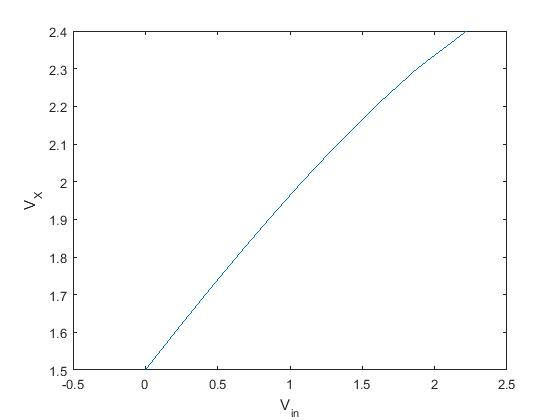
\includegraphics[width=10cm]{Q2_a_1.jpg}
 \caption{Q2\_a}
\end{figure}
\subsection*{b}
\begin{equation}
\frac{W}{L} = 0.8029
\end{equation}

\section*{Q3}
\subsection*{a}
It is clear that \begin{math}V_{X, max} = V_{DD} - V_{Th}\end{math}. And
\begin{equation}
 \begin{split}
  V_{Th} &= V_{T0} + \frac{1}{2}\gamma(\sqrt{2|\phi_F| + V_{X, max}/2} -\sqrt{2|\phi_F|})\\
  &=0.53(V)
 \end{split}
\end{equation}
Thus, \begin{math}V_{X, max}=1.97(V)\end{math}. As well as
\begin{equation}
 \begin{split}
  R_{eq}=& \frac{1}{2} R_{eq, max}\\
  =& \frac{V_{DD}-\frac{V_{X, max}}{2}}{\kappa\frac{W}{L}(V_{DD}-V_{X,max}/2 -V_{Th})^2 [1+\lambda(V_{DD}-V_{X, max}/2)]}\\
  =& 829.7861(\Omega)
 \end{split}
\end{equation}
Thus,
\begin{equation}
\begin{split}
t_{pLH} &= R_{eq}C_L ln\frac{V_{DD}}{V_{DD} - V_{out}}\\
&= R_{eq}C_L ln\frac{2V_{DD}}{V_{DD} + V_{Th}}\\
&= 2.0781(ns)
\end{split}
\end{equation}
\subsection*{b}
\begin{equation}
\begin{split}
\Delta t_{pLH} &= 0.69R_{eq}C_0 W_0\\
&= t_0
\end{split}
\end{equation}
\subsection*{c}
\begin{equation}
\begin{split}
t_{pHL} &= 0.69RC_L\\
& = 17.25 (ns)
\end{split}
\end{equation}
\subsection*{d}
With \begin{math}\beta_n = \beta_p\end{math}, and \begin{math}|\gamma_n| = |\gamma_p|\end{math} with 
\begin{math}|\lambda_n| = |\lambda_p|\end{math} from the table coming with questions.
\begin{math}\frac{t_{pLH, n}}{t_{pLH, p}}\end{math} becomes,
\begin{equation}
 \begin{split}
  \frac{t_{pLH, n}}{t_{pLH, p}} &= \frac{R_{eq, n}}{R_{eq, p}}\frac{ln\frac{2V_{DD}}{V_{DD} + V_{Tn}}}{ln\frac{2V_{DD}}{V_{DD} + 
  V_{Tp, 0}}} \\
  &= \frac{(V_{DD}+V_{Tn})(V_{DD}-V_{Tp, 0})^2 [1+\frac{1}{2}\lambda_p(V_{DD}+V_{Tp, 0})]ln\frac{2V_{DD}}{V_{DD} + V_{Tn}}}
  {(V_{DD}+V_{Tp, 0})(V_{DD}-V_{Tn})^2 [1+\frac{1}{2}\lambda_n(V_{DD}+V_{Tn})]ln\frac{2V_{DD}}{V_{DD} + V_{Tp, 0}}}\\
  &=1.1458
 \end{split}
\end{equation}
Which means, using PMOS will make it a bit faster.
\section*{Q4}
As how to use HSPICE is not taught, and therefore no tutorial was given. And this is the first time ever I've such a program, which
means there is no way I could know how to use it before hand. I can only use what I can see from netlist figures.
\subsection*{a}
For \begin{math}V_{M} = 0.5V_{DD}\end{math}, \begin{math}\frac{W_n}{W_p} = \frac{90}{127.50575} \approx \frac{90}{127.5}\end{math}.\\
\begin{tabular}{c|c}
 90/90	&	0.5576\\
 90/100	&	0.5715\\
 90/110	&	0.5819\\
 90/120	&	0.5925\\
 90/127.5	&	0.6\\
 90/140	&	0.6116\\
 90/150	&	0.6202\\
 90/160	&	0.6283\\
 90/170	&	0.6357\\
\end{tabular}
\begin{figure}
 \centering
 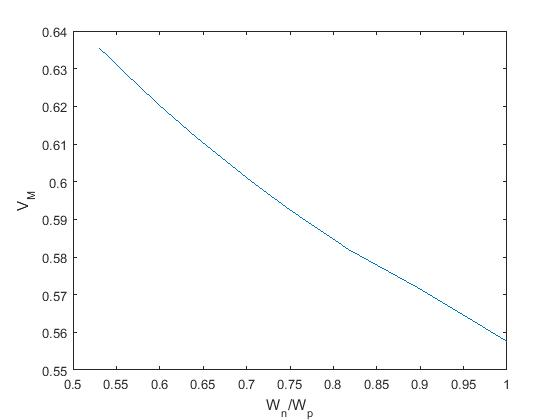
\includegraphics[width=10cm]{Q4_a.jpg}
 \caption{Q4\_a}
\end{figure}
\subsection*{b}
See Figure 3.\\
For high-to-low delay equals low-to-high delay, \begin{math}\frac{W_n}{W_p} = \frac{90}{135.75}\end{math}.\\
\begin{figure}
 \centering
 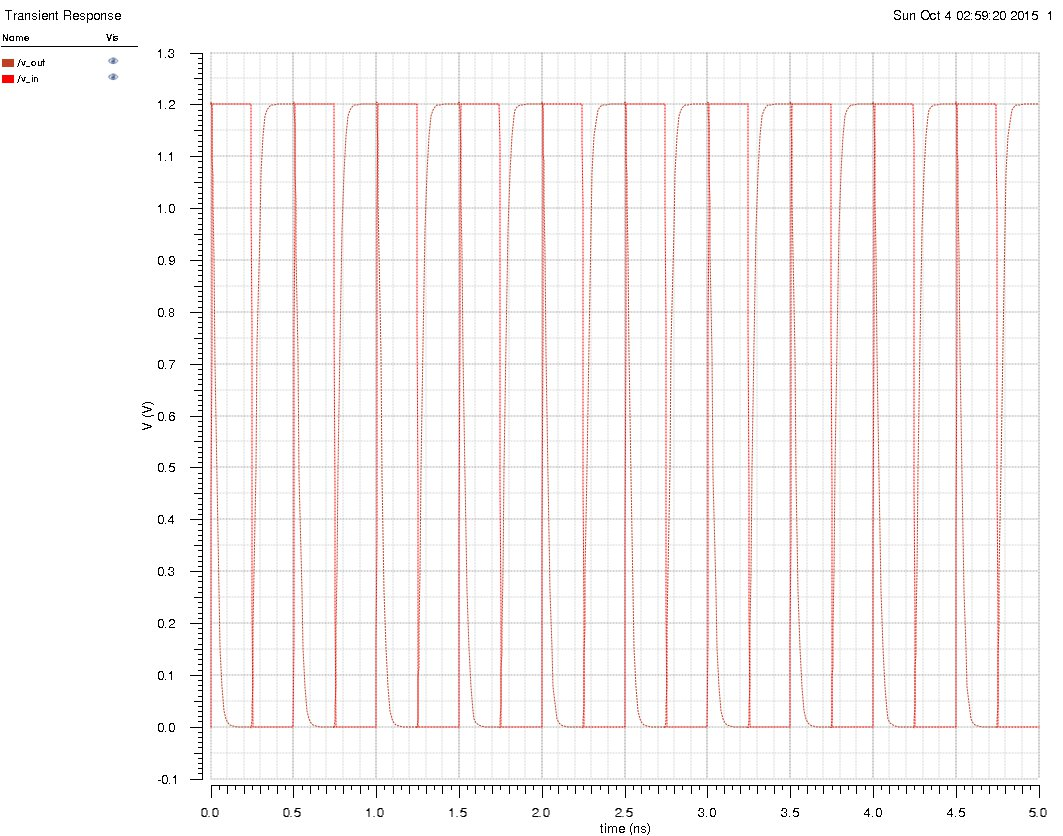
\includegraphics[width=10cm]{Q4_b.jpg}
 \caption{Q4\_b}
\end{figure}

\subsection*{c}
See Figure 4.\\

\begin{tabular}{c c c}
 D\_input(ps)	&	t\_pHL(ps)	&	t\_pLH(ps)\\
 0.1		&	27		&	27\\
 50		&	32		&	27\\
 100		&	39		&	27\\
 150		&	44		&	27\\
 200		&	48		&	27\\
 500		&	65		&	27\\
\end{tabular}
\begin{figure}
 \centering
 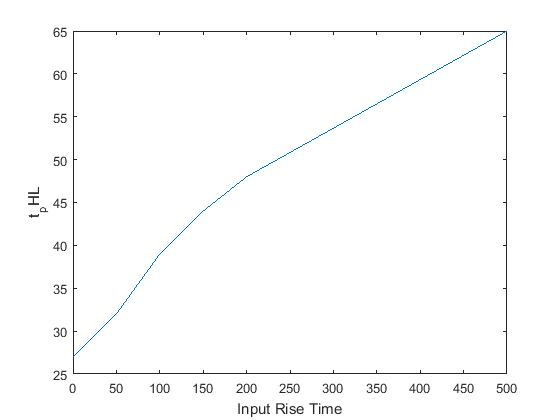
\includegraphics[width=10cm]{Q4_c.jpg}
 \caption{Q4\_c}
\end{figure}
\\
Quite clear that high-to-low delay is positively related with input rise time. And in fact it is still a fuction of input.
\subsection*{d}
Except for high-to-low delay increased to 67ps, I saw no suspicious things. And here is my paramiters:\\
\begin{tabular}{c l l}
 PMOS	&	L	&	50nm\\
	&	W	&	542.8nm\\
 NMOS	&	L	&	50nm\\
	&	W	&	90nm\\
 V\_dd	&		&	1.2V\\
 V\_in	&	rise time	&	200ps\\
	&	fall time	&	10ps\\
	&	pulse width	&	235ps\\
	&	period	&	880ps\\
	&	voltage 1	&	0V\\
	&	voltage 2	&	1.2V\\
 Cap	&		&	5fF\\
\end{tabular}
\subsection*{e}
For what I got, it is the same as the result from part (b). And have no conflict with part(c).
\begin{equation}
 \begin{split}
  \frac{t_{pHL}}{t_{pLH}} =& \frac{R_n}{R_p}\\
  =& \frac{I_{DSAT, p}(1-\frac{7}{9}\lambda_n V_{DD})}{I_{DSAT, N}(1-\frac{7}{9}\lambda_p V_{DD})}\\
  =& \frac{\kappa_p W_p (V_{DD} - V_{T0})^2 (1-\frac{7}{9}\lambda_n V_{DD})}{\kappa_n W_n (V_{DD} - V_{Tn})^2 (1-\frac{7}{9}\lambda_p V_{DD})}\\
 \end{split}
\end{equation}
Thus the ratio has nothing to do with input rise/fall time. But, ofcourse, signal frequency become too high, output will go
wild.
\end{document}
